\documentclass[sigconf, nonacm]{acmart}
\usepackage{tikz}
\usetikzlibrary{decorations.pathreplacing} % Acolades
\usetikzlibrary{arrows}
\usepackage{bm}

%% \BibTeX command to typeset BibTeX logo in the docs
\AtBeginDocument{%
  \providecommand\BibTeX{{%
    \normalfont B\kern-0.5em{\scshape i\kern-0.25em b}\kern-0.8epm\TeX}}}

%% If you are preparing content for an event
%% sponsored by ACM SIGGRAPH, you must use the "author year" style of
%% citations and references.
%% Uncommenting
%% the next command will enable that style.
%%\citestyle{acmauthoryear}

\begin{document}
\title{Towards Hierarchical Explanation}
\author{Christiaan van der Vlist}
\affiliation{
  %\institution{University of Amsterdam}
  %\country{Netherlands}
}
\email{christiaan.vandervlist@student.uva.nl}

\author{Albert Harkema}
\affiliation{%
  \institution{}
  \country{}}
\email{albert.harkema@student.uva.nl}

\author{Anna Langedijk}
\affiliation{%
  \institution{}
  \country{}
}
\email{annalangedijk@gmail.com}

\author{Hinrik Snær Guðmundsson}
\affiliation{%
 \institution{}
 \country{}}
 \email{hinriksnaer@gmail.com}
\renewcommand{\shortauthors}{van der Vlist, et al.}

%%
%% The abstract is a short summary of the work to be presented in the
%% article.
\begin{abstract}
Write a summary of our report. Writing this last.
\end{abstract}


\maketitle

% Welcome to our file!
% Please type the actual content of the paper in the tex files in the content/ directory
\section{Introduction}\label{sec:intro}
The importance of transparency in Machine Learning is rapidly increasing. As Machine Learning algorithms grow in prominence in society, being able to explain the decision making process of these algorithms in an intelligible manner has become more important. This is true both from a legal perspective (such as with the GDPR \citep{gdprart}) as from a human perspective -- interpretability engenders trust in users, even when it makes mistakes \citep{automtrust}, which is especially important when people rely on the algorithm to keep them healthy and safe, as is the case with medical AI or self-driving cars. Furthermore, an explainable algorithm allows us to better detect biases and spurious relationships present in the training data, e.g. because of data leakage \citep{dataleakage}. However, most modern Machine Learning algorithms rely on artificial neural networks which use nonlinearities to capture hidden relations between inputs and outputs. This makes explaining model output in a satisfactory way complex \cite{NNblackboxexplanation}.

A number of different approaches have been proposed to address the inherent lack of transparency prevalent in widely used neural network architectures. One example of those approaches is the explanation technique LIME \citep{LIME}, which provides local (i.e. for a single input) explanations of what features are important for the classification. When applied to images, for example, it highlights which pixels weighed heavily in its decision-making. This technique is binary -- a feature was either a relevant factor or not. Other examples of methods that focus on explanation through feature highlighting have been recently proposed by Lundburg \& Lee \citep{featureexamplepaper1}. One drawback of the methods of improving explanation discussed so far is that they require new models to be trained in order to make explanation possible. A method that does not have this issue is Integrated Gradients \citep{axioms}, which also does feature highlighting but can be applied to existing models.

A more specific method of explaining why a model classifies inputs in a certain way is by visualizing what a model considers to be an archetypal example of a given class. Activation Maximization (AM) \citep{activationmaximization} is such a method: for each class it provides a hypothetical input that would produce the highest activation for that class. However, from a human point of view, such inputs tend to be dissimilar to actual inputs from that class  \citep{activationmaximization}. This goes against our intuition that model explanations should be interpretable as well as accurate. To resolve this dissimilarity, Li et al. \citep{li2018deep} propose a representation learning architecture for a \textit{prototype classifier}. This architecture classifies by measuring distance between input and prototypes, which are defined as points that represent a class in a latent space. These are learned through regularization such that they are close to encoded inputs corresponding to that class. Li et al. simultaneously train this classifier and an autoencoder \citep{autoencoderpaper} that transforms inputs to the latent space of the prototypes. After training has finished, the autoencoder can be used to visualize the prototypes by decoding them.

In this paper, we first of all attempt to reproduce the results attained by the architecture introduced by Li et al. \citep{li2018deep}. Secondly, we extend the architecture with hierarchical prototypes. This hierarchy is composed of two layers: superprototypes and subprototypes. Subprototypes are close to actual encoded input (similar to prototypes in the original architecture), while superprototypes act as descriptors for the subprototype clusters in the latent space. For example, when training on the MNIST dataset, subprototypes can find different ways of writing the same digit (as prototypes do in \citep{li2018deep}), while superprototypes come to represent the average way numbers are written. By visualizing the sub- and superprototypes an encoded input is closest to, we gain an extra layer of interpretability for the classification process. When the number of superprototypes is equal to the number of classes, a fixed activation pattern based on closest superprototype can be used to force the detection of all classes. The subprototypes will in this case take care of intraclass variation. The network automatically learns which classes need more subprototypes: in MNIST terminology, there may be more distinct ways to write a 2 than there are ways to write a 9. This solves an issue that the original architecture \citep{li2018deep} had, namely that when the number of prototypes exceeded the number of classes, there were cases where not all classes were represented by a prototype (for an example, see Figure~\ref{fig:non3} in the Appendix).

In the next section, we will briefly explain the original, nonhierarchical architecture. This is followed by a detailed description of our hierarchical prototype network. In Section~\ref{sec:setup}, we describe and justify our choice of hyperparameters. Results for both reproduction and the new architecture are examined in Section~\ref{sec:results}, followed by a discussion of both the benefits and shortcomings of (hierarchical) prototype networks. Finally, Section~\ref{sec:broad} discusses some broader implications within the field of transparancy and fairness in artificial intelligence. 


\section{Method}\label{sec:method}
\begin{itemize}
    \item Explain in detail how the algorithm works (and how we ported it from tensorflow to pytorch).
    \begin{itemize}
        \item Show the architecture image from the original paper.
    \end{itemize}
    \item Explain how we extended it for our experiment.
\end{itemize}

The original architecture from \citep{li2018deep} is comprised of two parts. These are an autoencoder and a prototype network. The autoencoder's encoder, $f$, takes a $p$-dimensional input $\textbf{x}$ and transforms it to a $q$-dimensional latent-space. The decoder, $g$, takes a $q$-dimensional input and transforms it back into $p$-dimensional space. The prototype network, $h$, takes a $q$-dimensional input and outputs $K$ probabilities, one for each of the $K$ classes. This network itself consists of a prototype layer $p : \mathbb{R}^q\rightarrow\mathbb{R}^m$, followed by a fully-connected linear layer $w : \mathbb{R}^m\rightarrow\mathbb{R}^K$ with learnable weights (unless $m = K$, see further down), and finally a softmax layer $s : \mathbb{R}^K\rightarrow\mathbb{R}^K$. The prototype layer contains $m$ learnable $q$-dimensional prototype vectors. When given an input, this layer calculates the squared $L^2$ distance between this input and each of the prototype vectors. These distances are then pushed through $w$ and then through $s$ to get the classification. In case $m = K$, $w$ is a negative identity matrix $-I_{K \times K}$ instead.

The loss is comprised of a sum of four terms: Cross-entropy for the classification, the reconstruction error of the autoencoder, and two interpretability terms $R_1$ and $R_2$, defined as the mean of the minimum of squared $L^2$ distances between every prototype and all encoded inputs and between every encoded input and all prototypes respectively. Hyperparameters can be used to set the ratio between these terms.

\section{Experimental setup}\label{sec:setup}
Describe the setup (hyperparameters etc) and why we chose those. For the MNIST this probably boils down to that we copied the original paper. For the new dataset we have to be more verbose.

Because our first goal is to reproduce the results attained by \cite{li2018deep} we used the hyperparameters that are used in the paper. The authors set a number of hyperparameters: the number of prototype vectors, the size of the latent space and four hyperparameters $\lambda_{\text{class}}$, $\lambda_{\text{ae}}$, $\lambda_1$ and $\lambda_2$ for adjusting the ratio between the reconstruction error, the R1 term and the R2 term respectively. To allow for reproducibility, we used values of 20, 1, 1, and 1 respectively as done by \cite{li2018deep}.

Furthermore, for the training we set the learning rate to 0.0001, the amount of epochs to 1500 and the batch size to 250 in accordance with with \cite{li2018deep}. This fairly low learning rate allows for slow but steady convergence but also necessitates a fairly high number of epochs, hence the usage of 1500 epochs. 

\section{Results}\label{sec:results}
This is just a test! Feel free to remove it.



\section{Discussion}\label{sec:discussion}
\begin{itemize}
    \item Were we able to reproduce the original paper's results?
    \item What are the pros and cons of this algorithm. Can the cons be compensated for? How do these pros and cons relate to what problems this algorithm is useful for?
    \item What other datasets/problems should this algorithm be tested on?
\end{itemize}

\section{Broader Implications}\label{sec:broad}
Our primary goal is to provide an architecture that is both accurate and interpretable, which places our architecture within the domains of Transparency and Accountability. Another domain that has been getting more attention recently, however, is that of Fairness. Algorithms can be considered fair if they do not give disparate treatment to a certain disadvantaged group. Fairness criteria that are supposed to effect this are, according to \citet{fairnessgeneral}, "clearly intended to protect the disadvantaged group", even though they are not always succesful in improving the well-being of the this group \citep{fairnessgeneral}.

An important part of fairness is determining which algorithms are actually fair and which are biased. Bringing these biases to light in existing models has led, for example, to reduced disparity in hiring processes \citep{accountabilitycompanies}. Exposing biases is something that interpretable models aid in. In the case of the architecture of \citet{li2018deep} and our own architecture, for example, prototypes provide archetypical examples of data classes. When applied to, say, hiring data, prototypes show if the archetypical person that gets hired tends to be of a certain gender, race, or other sensitive category. If a model is found to be biased, appropriate action can be taken.

On the other hand, our architecture is not capable of downplaying or removing certain information from the input. This is necessary if the architecture is to be used for fair classification that does not rely on sensitive information present in the input. Simply removing features explicitly related to this sensitive information is not enough, since the information can be inferred from other correlated features \citep{unawarenesssucks}.

Both interclass and intraclass differences may be used to check for biases in the model or the data it is trained on. A certain class may be underrepresented when it has few subprototypes, or may have a much higher variance in its subprototypes. Although these variations are not related to fairness when it comes to MNIST digits, they may become relevant when a prototype network is trained on data containing sensitive information. P

A variant of the variational autoencoder architecture \citep{vae} proposed by Louizos et al. \citep{vfae} is capable of transforming input to a latent space in such a way that information can be factored out of the latent representation, while maintaining as much information as possible that is useful for classification. One potential way of making the architecture we propose in this paper fairer is by replacing the autoencoder with a Variational Fair Autoencoder. The prototypes would also need to be changed from points to distributions in the latent space. We believe that this will result in prototypes that are unbiased toward the sensitive information.



\section{Conclusion}\label{sec:conclusion}
\begin{itemize}
    \item Write conclusionesque stuff.
    \item Give an ACM badge to the algorithm (a what? I don't know either).
\end{itemize}

%%% Local Variables:
%%% mode: latex
%%% TeX-master: t
%%% End:


%%
%% The next two lines define the bibliography style to be used, and
%% the bibliography file.
\bibliographystyle{ACM-Reference-Format}
\bibliography{our_bibliography}

\newpage
\section*{Appendix}
\begin{figure}[!h]
    \centering
    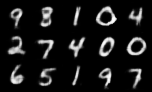
\includegraphics{img/reproduced9.png}
    \caption{Reproduced prototypes with seed set to 9. Notice that there is no prototype learned for class 3.}
    \label{fig:non3}
\end{figure}

\end{document}
\endinput
%%
%% End of file `sample-sigconf.tex'.

%%% Local Variables:
%%% mode: latex
%%% TeX-master: t
%%% End:
